\begin{center}
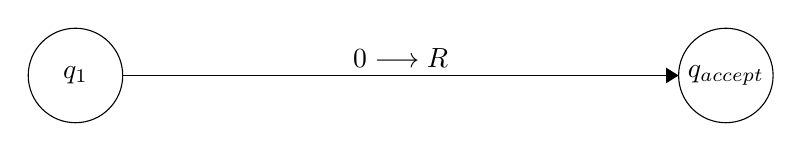
\begin{tikzpicture}[scale=0.2]
\tikzstyle{every node}+=[inner sep=0pt]
\draw [black] (18.7,-29.1) circle (3);
\draw (18.7,-29.1) node {$q_1$};
\draw [black] (60,-29.1) circle (3);
\draw (60,-29.1) node {$q_{accept}$};
\draw [black] (21.7,-29.1) -- (57,-29.1);
\fill [black] (57,-29.1) -- (56.2,-28.6) -- (56.2,-29.6);
\draw (39.35,-28.6) node [above] {$0\longrightarrow R$};
\end{tikzpicture}
\end{center}
